\chapter{Introduction}

\epigraph{The stars are not lonely, in their shining solitude. They have each other, and they have us.}{Isaac Asimov, "The Stars, Like Dust"}


Observations proved that field stars are not always single; many develop in pairs, and many of these binaries are members of triples or higher-order systems. Additionally, the fraction of systems with companions grows with mass (see \cref{fig:stellar_companions}), as a result massive stars are seldomly formed in isolation. In contrast, most of massive stars are created in binary or higher order multiple systems with $\sim 50\%$ of spectral type B stars be in triples \citep{sana2014southern,moe2017mind}, a percentage which reduces to $\sim 10\%$ for low-mass stars \citep{raghavan2010survey,toonen2014popcorn,moe2017mind}. In these cases, apart from the intrinsic stellar properties, the evolution depends sensitively on the interaction between the system's stellar components. Consequently, triple systems are not as uncommon as we may mistakenly believe, particularly in the concept of massive stars, the life cycle of which is still poorly understood.

Although the fundamentals of single and binary evolution have long been acknowledged \citep{postnov2014evolution,toonen2014popcorn}, the long-term evolution of stellar triples remains unknown. In the simple case, stable triple systems, which are hierarchical, namely, consist of an inner and an outer binary orbit, i.e., the tertiary (third object). The secular evolution of such systems is the modification of orbital elements over timescales substantially larger than the system's dynamical timescale. Hence, the presence of the outer star has no influence on the history of the inner binary and the evolution of the inner binary and the tertiary can be discussed independently. In other cases, a third star in orbit around a binary system can drastically influence the system's development
via dynamical interactions, which influence the orbital elements of the inner and outer orbit through changes in energy and angular momentum. Consequently, hierarchical triple star systems can become unstable via triple stellar evolution processes which are unique to systems with multiplicities of higher orders than binaries.
\begin{figure}[H]
    \centering
    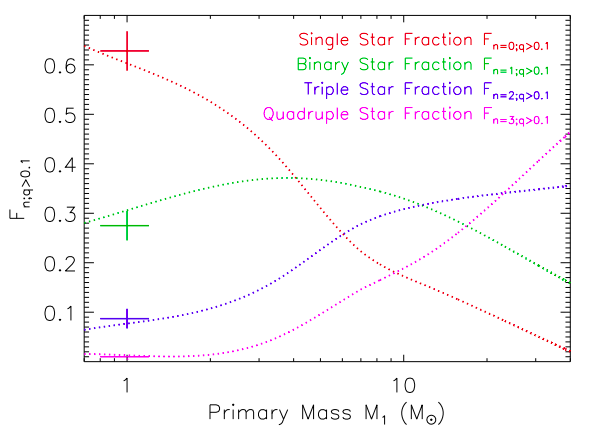
\includegraphics[width=\textwidth]{Thesis/figures/fig_moe_2017.png}
    \caption{Multiplicity fractions as a function of primary mass (dotted lines), including the single-star $F_{n=0;q> 0.1}$ (red), binary-star $F_{n=1;q> 0.1}$  (green), triple-star $F_{n=2;q> 0.1}$  (blue), and quadruple-star fraction $F_{n=3;q> 0.1}$  (magenta). Given a primary mass $M_1$, the model assumes that the multiplicity fractions follow a Poisson distribution across the interval $n = [0, 3]$ in a manner that reproduces the measured multiplicity frequency $F_{mult;q >0.1} = \Sigma_{n=1}^3 \; n F_{n;q> 0.1}$. For solar-type stars, this model matches the measured values (solid) within their uncertainties. Regardless of the uncertainties in the multiplicity fractions, $\leq 10\%$ of O-type stars are single while $\geq 55\%$ are born in triples and/or quadruples. Figure taken by \cite{moe2017mind}.}
    \label{fig:stellar_companions}
\end{figure}
The rich dynamical behavior of three-body systems can produce Lidov-Kozai cycles, in which the eccentricity of the inner orbit and the inclination between the inner and outer orbits vary periodically \citep{michaely2014secular,toonen2016evolution,mangipudi2022extreme}. As a result, tidal effects (tidal friction), gravitational-wave emission, and stellar interactions such as mass transfer, angular momentum exchange and collisions may be enhanced. In this way, evolution in triples can give rise to stellar mergers \citep{antonini2017binary,silsbee2017lidov,vigna2021massive}, namely some of most energetic events in the universe, ranging from gravitational wave sources to electromagnetic transients, e.g. luminous red novae, and also provide promising evolutionary pathways for exotic objects \citep{sana2012binary, toonen2016evolution}, e.g. blue stragglers \citep{winn2009spin}. In the past, most of our efforts in understanding the progenitors of the events were focused on modeling binary evolution disregarding the interaction of the binary with a third star. Therefore, a detailed examination of triple evolution is as necessary as it is challenging because it demands a self consistent treatment of three-body dynamics and stellar evolution.

\section{Goal \& Scientific Questions}

In this thesis, I present the evolution of TIC 470710327 \citep{eisner2022planet}, a massive hierarchical triple system with a Roche lobe filling outer star. I use the Astrophysical Multipurpose Software Environment (AMUSE, \cite{pelupessy2013astrophysical,portegies2018astrophysical}) to simulate the system's evolution and try to predict its future. Initially, I create stellar evolution models of the triple components until the tertiary fills its Roche lobe. I then simulate in detail the mass transfer for several orbits of the outer star using a combination of gravitational dynamics and hydrodynamics. 

There are two main scientific questions that I try to tackle:

\begin{itemize}
    \item How the mass transfer affects the orbital parameters of the two orbits?
    \item How the accretion of the binary affects the orbital parameters of the two orbits?
\end{itemize}

I examine the importance of various parameters, properties and type of mass transfer, the response of the inner and outer orbital parameters, and the consequent evolution.





\section{Thesis Outline}
This thesis is structured as follows: 

In the second chapter, I present an overview of single massive star evolution until the end of helium burning phase with a focus on those aspects that are relevant for triple evolution. Furthermore, I discuss concepts of binary evolution and I argue how to extend these to the triple evolution case. In the remainder of this chapter, I provide information about the scientific codes utilized in my simulations. In chapter three, I introduce my target system. In the fourth chapter, I display the setup of my simulations, the underlying assumptions of my models, and their physical justification.



%\subsection{AMUSE}




